%iffalse
\let\negmedspace\undefined
\let\negthickspace\undefined
\documentclass[journal,12pt,onecolumn]{IEEEtran}
\usepackage{cite}
\usepackage{amsmath,amssymb,amsfonts,amsthm}
\usepackage{algorithmic}
\usepackage{graphicx}
\usepackage{textcomp}
\usepackage{xcolor}
\usepackage{txfonts}
\usepackage{listings}
\usepackage{enumitem}
\usepackage{mathtools}
\usepackage{gensymb}
\usepackage{comment}
\usepackage[breaklinks=true]{hyperref}
\usepackage{tkz-euclide} 
\usepackage{listings}
\usepackage{gvv}                                        
%\def\inputGnumericTable{}                                 
\usepackage[latin1]{inputenc}     
\usepackage{xparse}
\usepackage{color}                                            
\usepackage{array}                                            
\usepackage{longtable}                                       
\usepackage{calc}                                             
\usepackage{multirow}
\usepackage{multicol}
\usepackage{hhline}                                           
\usepackage{ifthen}                                           
\usepackage{lscape}
\usepackage{tabularx}
\usepackage{array}
\usepackage{float}
\newtheorem{theorem}{Theorem}[section]
\newtheorem{problem}{Problem}
\newtheorem{proposition}{Proposition}[section]
\newtheorem{lemma}{Lemma}[section]
\newtheorem{corollary}[theorem]{Corollary}
\newtheorem{example}{Example}[section]
\newtheorem{definition}[problem]{Definition}
\newcommand{\BEQA}{\begin{eqnarray}}
\newcommand{\EEQA}{\end{eqnarray}}
\usepackage{float}
%\newcommand{\define}{\stackrel{\triangle}{=}}
\theoremstyle{remark}
\usepackage{ circuitikz }
%\newtheorem{rem}{Remark}
% Marks the beginning of the document
\begin{document}
\title{CH: Chemical Engineering}
\author{EE25BTECH11012 - BEERAM MADHURI}
\maketitle
\renewcommand{\thefigure}{\theenumi}
\renewcommand{\thetable}{\theenumi}

\begin{enumerate}

\item Consider the following set of linear algebraic equations
\begin{align*}x_1 + 2x_2 + 3x_3 &= 2 \\x_2 + x_3 &= -1 \\2x_2 + 2x_3 &= 0\end{align*}
The system has
\hfill{\brak{\text{CH 2012}}}
\begin{enumerate}
\begin{multicols}{2}
\item a unique solution
\item no solution
\item an infinite number of solutions
\item only the trivial solution
\end{multicols}
\end{enumerate}

\item If $a$ and $b$ are arbitrary constants, then the solution to the ordinary differential equation
\[\frac{d^2 y}{dx^2} - 4y = 0\]
is
\hfill{\brak{\text{CH 2012}}}
\begin{enumerate}
\begin{multicols}{2}
\item $y = ax + b$ 
\item $y = ae^{-x}$
\item $y = a\sin 2x + b\cos 2x$
\item $y = a\cosh 2x + b\sinh 2x$
\end{multicols}
\end{enumerate}

\item For the function $f(t) = e^{-t/\tau}$,
the Taylor series approximation for $t \ll \tau$ is
\hfill{\brak{\text{CH 2012}}}
\begin{enumerate}
\begin{multicols}{4}
\item $1 + \frac{t}{\tau}$ 
\item $1 - \frac{t}{\tau}$
\item $1 - \frac{t^2}{2\tau^2}$
\item $1 + t$
\end{multicols}
\end{enumerate}

\item A box containing 10 identical compartments has 6 red balls and 2 blue balls. If each compartment can hold only one ball, then the number of different possible arrangements are
\hfill{\brak{\text{CH 2012}}}
\begin{enumerate}
\begin{multicols}{4}
\item $1026$ 
\item $1062$
\item $1260$
\item $1620$ 
\end{multicols}
\end{enumerate}

\item Consider the following $(2\times 2)$ matrix
\[\begin{pmatrix}4 & 0 \\0 & 4\end{pmatrix}.\]
Which one of the following vectors is NOT a valid eigenvector of the above matrix?
\hfill{\brak{\text{CH 2012}}}
\begin{enumerate}
\begin{multicols}{4}
\item $\begin{pmatrix} 1 \\ 0 \end{pmatrix}$
\item $\begin{pmatrix} -2 \\ 1 \end{pmatrix}$ \\
\item $\begin{pmatrix} 4 \\ -3 \end{pmatrix}$
\item $\begin{pmatrix} 0 \\ 0 \end{pmatrix}$
\end{multicols}
\end{enumerate}

\item In a throttling process, the pressure of an ideal gas reduces by $50\%$. If $C_p$ and $C_V$ are the heat capacities at constant pressure and constant volume, respectively ($\gamma = C_p/C_V$), the specific volume will change by a factor of
\hfill{\brak{\text{CH 2012}}}
\begin{enumerate}
\begin{multicols}{4}
\item $2$
\item $2^{\gamma}$ 
\item $2^{\gamma-1/\gamma}$
\item $0.5$
\end{multicols}
\end{enumerate}

\item In a throttling process, the pressure of an ideal gas reduces by $50\%$. If $C_p$ and $C_V$ are the heat capacities at constant pressure and constant volume, respectively ($\gamma = C_p/C_V$), the specific volume will change by a factor of
\hfill{\brak{\text{CH 2012}}}
\begin{enumerate}
\begin{multicols}{4}
\item $2$
\item $2^{\gamma}$
\item $2^{\gamma-1/\gamma}$
\item $0.5$
\end{multicols}
\end{enumerate}

\item In a parallel flow heat exchanger operating under steady state, hot liquid enters at a temperature $T_{h,in}$ and leaves at a temperature $T_{h,out}$. Cold liquid enters at a temperature $T_{c,in}$ and leaves at a temperature $T_{c,out}$. Neglect any heat loss from the heat exchanger to the surrounding. If $T_{h,in} \gg T_{c,in}$, then for a given time interval, which ONE of the following statements is true?
\hfill{\brak{\text{CH 2012}}}
\begin{enumerate}
\item Entropy gained by the cold stream is GREATER than entropy lost by the hot stream 
\item Entropy gained by the cold stream is EQUAL to the entropy lost by the hot stream 
\item Entropy gained by the cold stream is LESS than the entropy lost by the hot stream
\item Entropy gained by the cold stream is ZERO
\end{enumerate}

\item For an exothermic reversible reaction, which one of the following correctly describes the dependence of the equilibrium constant ($K$) with temperature ($T$) and pressure ($P$) ?
\hfill{\brak{\text{CH 2012}}}
\begin{enumerate}
\item $K$ is independent of $T$ and $P$
\item $K$ increases with an increase in $T$ and $P$
\item $K$ increases with $T$ and decreases with $P$
\item $K$ decreases with an increase in $T$ and is independent of $P$
\end{enumerate}

\item Water is flowing under laminar conditions in a pipe of length $L$. If the diameter of the pipe is doubled, for a constant volumetric flowrate, the pressure drop across the pipe
\hfill{\brak{\text{CH 2012}}}
\begin{enumerate}
\begin{multicols}{2}
\item decreases 2 times
\item decreases 16 times
\item increases 2 times 
\item increases 16 times
\end{multicols}
\end{enumerate}

\item The local velocity of a fluid along a streamline can be measured by
\hfill{\brak{\text{CH 2012}}}
\begin{enumerate}
\begin{multicols}{4}
\item Pitot tube
\item Venturi meter
\item Rotameter
\item Orifice meter
\end{multicols}
\end{enumerate}

    \item For uniform laminar flow (in the $x$-direction) past a flat plate at high Reynolds number, the local boundary layer thickness ($\delta$) varies with the distance along the plate ($x$) as
    \hfill{\brak{\text{CH 2012}}}
    \begin{enumerate}
    \begin{multicols}{4}
        \item $\delta \propto x^{\frac{1}{4}}$
        \item $\delta \propto x^{\frac{1}{2}}$
        \item $\delta \propto x^{\frac{4}{5}}$
        \item $\delta \propto x$
  \end{multicols}
  \end{enumerate}

    \item In a mixing tank operating at very high Reynolds number ($> 10^4$), if the diameter of the impeller is doubled (other conditions remaining constant), the power required increases by a factor of
    \hfill{\brak{\text{CH 2012}}}
    \begin{enumerate}
    \begin{multicols}{4}
        \item $1/32$
        \item $1/4$
        \item $4$
        \item $32$
        \end{multicols}
    \end{enumerate}

    \item For heat transfer across a solid-fluid interface, which one of the following statements is NOT true when the Biot number is very small compared to 1?
    \hfill{\brak{\text{CH 2012}}}
    \begin{enumerate}
        \item Conduction resistance in the solid is very small compared to convection resistance in the fluid
        \item Temperature profile within the solid is nearly uniform
        \item Temperature drop in the fluid is significant
        \item Temperature drop in the solid is significant
    \end{enumerate}

    \item A solid sphere with an initial temperature $T_i$ is immersed in a large thermal reservoir of temperature $T_0$. The sphere reaches a steady temperature after a certain time $t_1$. If the radius of the sphere is doubled, the time required to reach steady-state will be
    \hfill{\brak{\text{CH 2012}}}
    \begin{enumerate}
    \begin{multicols}{4}
        \item $t_1/4$
        \item $t_1/2$
        \item $2 t_1$
        \item $4 t_1$
        \end{multicols}
    \end{enumerate}

    \item If the Nusselt number (Nu) for heat transfer in a pipe varies with Reynolds number (Re) as $\text{Nu} \propto \text{Re}^{0.8}$, then for constant average velocity in the pipe, the heat transfer coefficient varies with the pipe diameter $D$ as
    \hfill{\brak{\text{CH 2012}}}
    \begin{enumerate}
    \begin{multicols}{4}
        \item $D^{-1.8}$
        \item $D^{-0.2}$
        \item $D^{0.2}$
        \item $D^{1.8}$
        \end{multicols}
    \end{enumerate}

    \item In the McCabe-Thiele diagram, if the $x$-coordinate of the point of intersection of the $q$-line and the vapor-liquid equilibrium curve is greater than the $x$-coordinate of the feed point, then the quality of the feed is
    \hfill{\brak{\text{CH 2012}}}
    \begin{enumerate}
    \begin{multicols}{2}
        \item super-heated vapor
        \item liquid below bubble point
        \item saturated vapor
        \item saturated liquid
\end{multicols}
\end{enumerate}

    \item For which of the following combinations, does the absorption operation become gas-film controlled?
\hfill{\brak{\text{CH 2012}}}
    \begin{enumerate}
        \item[P.] The solubility of gas in the liquid is very high
        \item[Q.] The solubility of gas in the liquid is very low
        \item[R.] The liquid-side mass transfer coefficient is much higher than the gas-side mass transfer coefficient
        \item[S.] The liquid-side mass transfer coefficient is much lower than the gas-side mass transfer coefficient
    \end{enumerate}
    \begin{enumerate}
    \begin{multicols}{4}
        \item P \& Q
        \item P \& R
        \item P \& S
        \item Q \& R
    \end{multicols}
    \end{enumerate}

    \item The half-life of an $n^{\text{th}}$ order reaction in a batch reactor depends on
    \hfill{\brak{\text{CH 2012}}}
    \begin{enumerate}
        \item only the rate constant
        \item only the rate constant and the order of the reaction
        \item only the rate constant and the initial reactant concentration
        \item the rate constant, initial reactant concentration, and the
\end{enumerate}

\item Consider the reaction scheme shown below
\[A \xrightarrow{k_1} B \xrightarrow{k_2} C.\]
Both the reactions are first-order. The activation energies for $k_1$ and $k_2$ are $80$ kJ/mol, respectively. To maximize the yield of B, it is preferable to use
\hfill{\brak{\text{CH 2012}}}
\begin{enumerate}
    \item CSTR and high temperature
    \item PFR and high temperature
    \item CSTR and low temperature
    \item PFR and low temperature
\end{enumerate}

\item In petroleum refining, catalytic reforming is used to convert
\hfill{\brak{\text{CH 2012}}}
\begin{enumerate}
    \item Paraffins and naphthenes to aromatics
    \item Paraffins to hydrogen and carbon monoxide
    \item Gas oil to diesel and gasoline
    \item Light olefins to gasoline
\end{enumerate}

\item The final boiling points of gasoline, diesel, atmospheric gas oil (AGO) and lubricating oils vary as
\hfill{\brak{\text{CH 2012}}}
\begin{enumerate}
    \item gasoline $>$ diesel $>$ AGO $>$ lubricating oils
    \item lubricating oils $>$ AGO $>$ diesel $>$ gasoline
    \item AGO $>$ lubricating oils $>$ diesel $>$ gasoline
    \item lubricating oils $>$ diesel $>$ AGO $>$ gasoline
\end{enumerate}

\item The main unit processes used for the production of hydrogen from natural gas are steam reforming (SR), pressure swing adsorption (PSA), low temperature water gas shift reaction (LT WGS) and high temperature water gas shift reaction (HT WGS). The correct sequence of these in the plant is
\hfill{\brak{\text{CH 2012}}}
\begin{enumerate}
    \item SR; LT WGS; HT WGS; PSA
    \item PSA; SR; LT WGS; HT WGS
    \item SR; HT WGS; LT WGS; PSA
    \item PSA; HT WGS; LT WGS; SR
\end{enumerate}
\item A thermometer initially at $100^\circ$C is dipped at $t = 0$ into an oil bath, maintained at $150^\circ$C. If the recorded temperature is $130^\circ$C after 1 minute, then the time constant of thermometer (in min) is
\hfill{\brak{\text{CH 2012}}}
\begin{enumerate}
\begin{multicols}{4}
    \item $1.98$
    \item $1.35$
    \item $1.26$
    \item $1.09$
    \end{multicols}
\end{enumerate}

\item The Bode stability criterion is applicable when
\hfill{\brak{\text{CH 2012}}}
\begin{enumerate}
    \item Gain and phase curves decrease continuously with frequency
    \item Gain curve increases and phase curve decreases with frequency
    \item Gain curve and phase curve both increase with frequency
    \item Gain curve decreases and phase curve increases with frequency
\end{enumerate}

\item The one-dimensional unsteady state heat conduction equation in a hollow cylinder with a constant heat source $q$ is
\[\frac{\partial T}{\partial t} = \frac{1}{r} \frac{\partial}{\partial r} \left( r \frac{\partial T}{\partial r} \right) + q\]
If $A$ and $B$ are arbitrary constants, then the steady state solution to the above equation is
\hfill{\brak{\text{CH 2012}}}
\begin{enumerate}
\begin{multicols}{2}
    \item $T(r) = -\frac{qr^2}{4} + A \ln r + B$
    \item $T(r) = -\frac{qr^2}{4} + A \ln r + B$
    \item $T(r) = A \ln r + B$
    \item $T(r) = \frac{qr^2}{4} + A \ln r + B$
    \end{multicols}
\end{enumerate}

\item If $a$ is a constant, then the value of the integral $\int_{0}^{\infty} x e^{-ax} dx$ is
\hfill{\brak{\text{CH 2012}}}
\begin{enumerate}
\begin{multicols}{4}
    \item $1/a$
    \item $a$
    \item $1$
    \item $0$
    \end{multicols}
\end{enumerate}

\item The Newton-Raphson method is used to find the roots of the equation
\[f(x) = x - \cos \pi x \quad 0 \leq x \leq 1.\]
If the initial guess for the root is $0.5$, then the value of $x$ after the first iteration is
\hfill{\brak{\text{CH 2012}}}
\begin{enumerate}
\begin{multicols}{4}
    \item $1.02$
    \item $0.62$
    \item $0.55$
    \item $0.38$
    \end{multicols}
\end{enumerate}

\item If $i = \sqrt{-1}$, the value of the integral
\[\oint \frac{2z + i}{z(z^2 + 1)} dz \quad |z| < 2,\]
using the Cauchy residue theorem is
\hfill{\brak{\text{CH 2012}}}
\begin{enumerate}
\begin{multicols}{4}
    \item $2\pi i$
    \item $0$
    \item $-6\pi$
    \item $6\pi$
    \end{multicols}
\end{enumerate}

\item An insulated, evacuated container is connected to a supply line of an ideal gas at pressure $P_s$, temperature $T_s$ and specific volume $v_s$. The container is filled with the gas until the pressure in the container reaches $P_s$. There is no heat transfer between the supply line to the container, and kinetic and potential energies are negligible. If $C_p$ and $C_v$ are the heat capacities at constant pressure and constant volume, respectively ($\gamma = C_p/C_v$), the final temperature of the gas in the container is
\hfill{\brak{\text{CH 2012}}}
\begin{enumerate}
\begin{multicols}{4}
    \item $\gamma T_s$
    \item $T_s$
    \item $(\gamma - 1)T_s$
    \item $(\gamma - 1)T_s/\gamma$
\end{multicols}
\end{enumerate}

\item Consider a binary liquid mixture at constant temperature $T$ and pressure $P$. If the enthalpy change of mixing, $\Delta H = 5x_1x_2$, where $x_1$ and $x_2$ are the mole fraction of species $1$ and $2$ respectively, and the entropy change of mixing $\Delta S = -R [x_1 \ln x_1 + x_2 \ln x_2]$ (with $R = 8.314$ J/mol.K), then the minimum value of the Gibbs free energy change of mixing at $300$ K occurs when
\hfill{\brak{\text{CH 2012}}}
\begin{enumerate}
\begin{multicols}{4}
    \item $x_1 = 0$
    \item $x_1 = 0.2$
    \item $x_1 = 0.4$
    \item $x_1 = 0.5$
\end{multicols}
\end{enumerate}

\item A bed of spherical glass beads (density $3000$ kg/m$^3$, diameter $1$ mm, bed porosity $0.5$) is to be fluidized by a liquid of density $1000$ kg/m$^3$ and viscosity $0.1$ Pas. Assume that the Reynolds number based on particle diameter is very small compared to one. If $g = 10$ m/s$^2$, then the minimum velocity (in m/s) required to fluidize the bed is
\hfill{\brak{\text{CH 2012}}}
\begin{enumerate}
\begin{multicols}{4}
    \item $3.33\times10^{-4}$
    \item $3.33\times10^{-1}$
    \item $3$
    \item $30$
    \end{multicols}
\end{enumerate}

\item For the enclosure formed between two concentric spheres as shown below ($R_{2} = 2R_{1}$), the fraction of radiation leaving the surface area $A_{2}$ that strikes itself is
\hfill{\brak{\text{CH 2012}}}
\begin{figure}[H]
    \centering
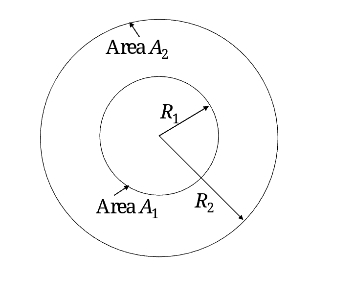
\includegraphics[width=0.25\columnwidth]{figs/qn 33 .jpg}
    \caption{}
    \label{fig:qn33.jpg}
\end{figure}
\begin{enumerate}
\begin{multicols}{4}
\item $1/4$
\item $1/2$
\item $\frac{1}{\sqrt{2}}$ 
\item $3/4$
\end{multicols}
\end{enumerate}

\item Heat is generated at a steady rate of $100 \, \text{W}$ due to resistance heating in a long wire (length = $5 \, \text{m}$, diameter = $2 \, \text{mm}$). This wire is wrapped with an insulation of thickness $1 \, \text{mm}$ that has a thermal conductivity of $0.1 \, \text{W/m.K}$. The insulated wire is exposed to air at $30^\circ\text{C}$. The convective heat transfer between the wire and surrounding air is characterized by a heat transfer coefficient of $10 \, \text{W/m}^2.\text{K}$. The temperature (in $^\circ\text{C}$) at the interface between the wire and the insulation is
\hfill{\brak{\text{CH 2012}}}
\begin{enumerate}
\begin{multicols}{4}
\item $211.2$ 
\item $242.1$ 
\item $311.2$
\item $484.2$
\end{multicols}
\end{enumerate}

\item In a counter-flow double pipe heat exchanger, oil ($\dot{m} = 2 \, \text{kg/s}$, $C_p = 2.1 \, \text{kJ/kg}.^\circ\text{C}$) is cooled from $90^\circ \, \text{C}$ to $40^\circ \, \text{C}$ by water ($\dot{m} = 1 \, \text{kg/s}$, $C_p = 4.2 \, \text{kJ/kg}.^\circ\text{C}$) which enters the inner tube at $10^\circ \, \text{C}$. The radius of the inner tube is $3 \, \text{cm}$ and its length is $5 \, \text{m}$. Neglecting the wall resistance, the overall heat transfer coefficient based on the inner radius, in $\text{kW/m}^2.\text{K}$, is
\hfill{\brak{\text{CH 2012}}}
\begin{enumerate}
\begin{multicols}{4}
\item $0.743$ 
\item $7.43$  
\item $74.3$
\item $2475$
\end{multicols}
\end{enumerate}

\item The rate-controlling step for the solid-catalyzed irreversible reaction
\[A + B \longrightarrow C\]
is known to be the reaction of adsorbed $A$ with adsorbed $B$ to give adsorbed $C$. If $P_i$ is the partial pressure of component $i$ and $K_i$ is the adsorption equilibrium constant of component $i$, then the form of the Langmuir-Hinshelwood rate expression will be
\hfill{\brak{\text{CH 2012}}}
\begin{enumerate}
\item  $\text{rate} \propto \frac{K_A K_B P_A P_B}{1+K_A P_A + K_B P_B + K_C P_C}$
\item $\text{rate} \propto \frac{P_A P_B}{(1+K_A P_A + K_B P_B + K_C P_C)^2}$

\item $\text{rate} \propto \frac{P_A P_B}{(1+K_A P_A + K_B P_B + K_C P_C)^{0.5}}$

\item $\text{rate} \propto \frac{P_A P_B}{P_C}$
\end{enumerate}

\item Consider the drying operation shown in the figure below for a solid loading (dry basis) of $50 \, \text{kg/m}^2$ with a constant drying rate of $5 \, \text{kg/m}^2.\text{h}$. The falling rate of drying is linear with moisture content.
\hfill{\brak{\text{CH 2012}}}
\[\begin{array}{c}X_c = 0.1 \\X_e = 0.005\end{array}\]
\begin{figure}[H]
    \centering
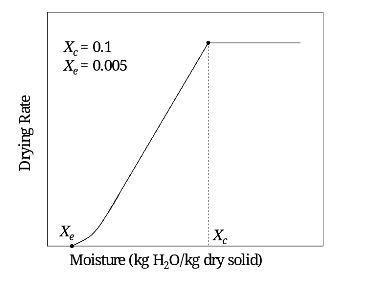
\includegraphics[width=0.3\columnwidth]{figs/qn 37.jpg}
    \caption{}
    \label{fig:qn.37.jpg}
\end{figure}

The drying time (in hrs) required to reduce an initial moisture content of $25\%$ to a final moisture content of $2\%$ is
\begin{enumerate}
\begin{multicols}{4}
\item $1.55$ 
\item $1.75$  
\item $3.25$
\item $4.55$
\end{multicols}
\end{enumerate}

\item An equimolar mixture of A and B (A being more volatile) is flash distilled continuously at a feed rate of $100 \, \text{kmol/h}$, such that the liquid product contains $40 \, \text{mol} \%$ of A. If the relative volatility is $6$, then the vapor product, in $\text{kmol/h}$ is
\hfill{\brak{\text{CH 2012}}}
\begin{enumerate}
\begin{multicols}{4}
    \item $10$
    \item $20$
    \item $25$
    \item $45$
    \end{multicols}
\end{enumerate}

\item A thermocouple having a linear relationship between $0 \, ^\circ\text{C}$ and $350 \, ^\circ\text{C}$ shows an emf of zero and $30.5 \, \text{mV}$, respectively at these two temperatures. If the cold junction temperature is shifted from $0 \, ^\circ\text{C}$ to $30 \, ^\circ\text{C}$, then the emf correction (in mV) is
\hfill{\brak{\text{CH 2012}}}
\begin{enumerate}
\begin{multicols}{4}
    \item $3.13$
    \item $2.92$
    \item $2.61$
    \item $2.02$
    \end{multicols}
\end{enumerate}

\item The characteristic equation for a system is
\[s^3 + 9s^2 + 26s + 12(2 + K_c) = 0.\]
Using the Routh test, the value of $K_c$ that will keep the system on the verge of instability is
\hfill{\brak{\text{CH 2012}}}
\begin{enumerate}
\begin{multicols}{4}
\item $20.9$
\item $18.4$ 
\item $17.5$ 
\item $15.3$
\end{multicols}
\end{enumerate}

\item The elementary reversible exothermic gas-phase reaction
\[A + 3B \rightleftharpoons 2C\]
is to be conducted in a non-isothermal, non-adiabatic plug flow reactor. The maximum allowable reactor temperature is $T_{\text{max}}$. To minimize the total reactor volume, the variation of reactor temperature ($T$) with axial distance from the inlet ($z$) should be
\hfill{\brak{\text{CH 2012}}}
\begin{figure}[H]
    \centering
    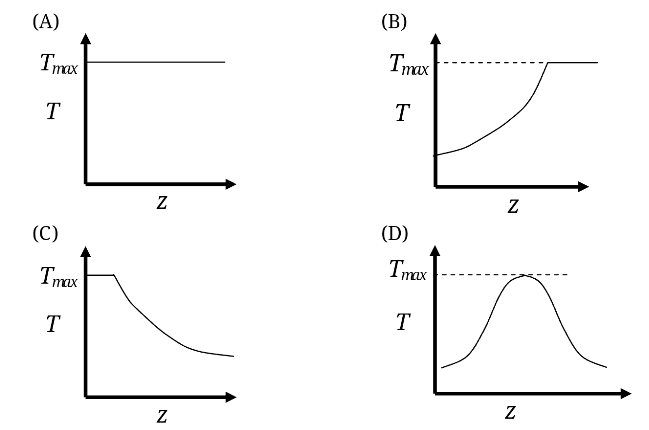
\includegraphics[width=0.65\columnwidth]{figs/qn 41.jpg}
    \caption{}
    \label{fig:qn41.jpg}
\end{figure}

\item The block diagram of a system with a proportional controller is shown below
\begin{figure}[H]
    \centering
    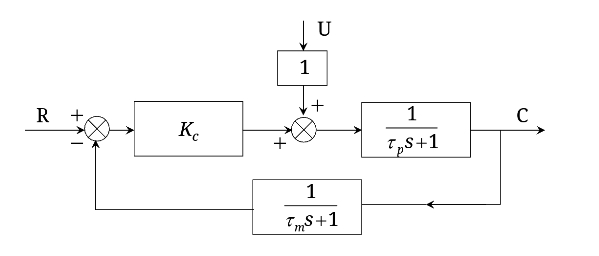
\includegraphics[width=0.4\columnwidth]{figs/qn 42 .jpg}
    \caption{}
    \label{fig:qn42.jpg}
\end{figure}
A unit step input is introduced in the set point. The value of $K_c$ to provide a critically damped response for $U = 0$, $\tau_p = 8$ and $\tau_m = 1$ is
\hfill{\brak{\text{CH 2012}}}

\begin{enumerate}
\begin{multicols}{4}
\item $3.34$
\item $2.58$
\item $1.53$
\item $1.12$
\end{multicols}
\end{enumerate}

\item A batch reactor produces $1 \times 10^5$ kg of a product per year. The total batch time (in hours) of the reactor is $k\sqrt{P_B}$, where $P_B$ is the product per batch in kg and $k = 1.0$ h/$\sqrt{\text{kg}}$. The operating cost of the reactor is Rs.200/h. The total annual fixed charges are Rs.$340 \times P_B$ and the annual raw material cost is Rs.~$2 \times 10^6$. The optimum size (in kg) of each batch (adjusted to the nearest integer) is
\hfill{\brak{\text{CH 2012}}}
\begin{enumerate}
\begin{multicols}{4}
\item $748$
\item $873$
\item $953$
\item $1148$
\end{multicols}
\end{enumerate}

\item Heat integration is planned in a process plant at an investment Rs.~$2\times10^6$. This would result in a net energy savings of 20 GJ per year. If the nominal rate of interest is 15\% and the plant life is 3 years, then the breakeven cost of energy, in Rs.~per GJ (adjusted to the nearest hundred), is
\hfill{\brak{\text{CH 2012}}}
\begin{enumerate}
\begin{multicols}{4}
\item $33500$
\item $43800$
\item $54200$
\item $65400$
\end{multicols}
\end{enumerate}

\item In a 1-1 pass floating head type shell and tube heat exchanger, the tubes (od = 25 mm, id = 21 mm) are arranged in a square pitch. The tube pitch is 32 mm. The thermal conductivity of the shell side fluid is 0.19 W/mK, and the Nusselt number is 200. The shell-side heat transfer coefficient (in W/m$^2$.K), rounded off to the nearest integer, is
\hfill{\brak{\text{CH 2012}}}
\begin{enumerate}
\begin{multicols}{4}
\item $1100$
\item $1400$
\item $1800$
\item $2100$
\end{multicols}
\end{enumerate}

\item & Match the process in \textbf{Group I} with the catalyst in \textbf{Group II}\\
\begin{tabular}{11}
\textbf{Group I} & \textbf{Group II} \\
P. Fischer-Tropsch synthesis & I. Nickel \\
Q. Formaldehyde from methanol & II. Fe$_2$O$_3$ \\
R. Hydrogenation of vegetable oils & III. Silver \\
S. Dehydrogenation of ethylbenzene  & IV. Cobalt \\
\end{tabular}
\hfill{\brak{\text{CH 2012}}}
\begin{enumerate}
\begin{multicols}{2}
\item[(A)] P-III, Q-IV, R-I, S-II
\item[(B)] P-IV, Q-II, R-I, S-III
\item P-IV, Q-III, R-I, S-II
\item P-III, Q-IV, R-II, S-I
\end{multicols}
\end{enumerate}

\item & Match the polymer in \textbf{Group I} to the polymer characteristic in \textbf{Group II}\\
\begin{tabular}{ll}
\textbf{Group I} & \textbf{Group II} \\
P. Polyethylene & I. Elastomer \\
Q. Phenol-formaldehyde polymer & II. Fiber \\
R. Polyisoprene & III. Thermoplastic \\
S. Polyester & IV. Thermosetting polymer \\
\end{tabular}
\hfill{\brak{\text{CH 2012}}}
\begin{enumerate}
\begin{multicols}{2}
\item P-III, Q-IV, R-I, S-II
\item P-IV, Q-II, R-III, S-I
\item P-III, Q-II, R-I, S-IV
\item P-IV, Q-III, R-I, S-II
\end{multicols}
\end{enumerate}

\section*{Common Data Questions}

\subsection*{Common Data for Questions 48 and 49}
A counter-current extraction column is designed to remove $99\%$ of solute C from a solution of solvent A and solute C using pure solvent B. The initial concentration of solute in the solution of A + C is $20$ wt $\%$, and the total flow of solution is $1000$ kg/h. If the equilibrium relationship is $Y = 2X$, where $Y =$ mass of C/mass of A and $X =$ mass of C/mass of B.

    \item The minimum flow rate of solvent B required (in kg/h) is
    \hfill{\brak{\text{CH 2012}}}
    \begin{enumerate}
    \begin{multicols}{4}
        \item $1454$
        \item $1584$
        \item $1676$
        \item $1874$
        \end{multicols}
        \end{enumerate}
    
    \item If the flow rate of B is $2400$ kg/h, then the theoretical number of stages in the column, using Kremser's equation (adjusted to the next integer) is
    \begin{enumerate}
    \hfill{\brak{\text{CH 2012}}}
    \begin{multicols}{4}
        \item $5$
        \item $9$
        \item $11$
        \item $13$
    \end{multicols}
    \end{enumerate}

\subsection*{Common Data for Questions 50 and 51}
The reaction $\text{A}{(\text{liq})} + \text{B}{(\text{gas})} \rightarrow \text{C}{(\text{liq})} + \text{D}{(\text{gas})}$, is carried out in a reactor followed by a separator as shown below
\hfill{\brak{\text{CH 2012}}}
\begin{figure}[H]
    \centering
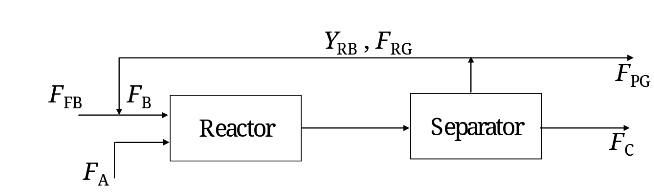
\includegraphics[width=0.5\columnwidth]{figs/qn 50 .jpg}
    \caption{}
\label{fig:qn51.jpg}
\end{figure}

\subsubsection*{Notation:}
\begin{itemize}
    \item Molar flow rate of fresh B is $F_{\text{FB}}$
    \item Molar flow rate of A is $F_{\text{A}}$
    \item Molar flow rate of recycle gas is $F_{\text{RG}}$
    \item Mole fraction of B in recycle gas is $Y_{\text{RB}}$
    \item Molar flow rate of purge gas is $F_{\text{PG}}$
    \item Molar flow rate of C is $F_{\text{C}}$
\end{itemize}

Here, $F_{\text{FB}} = 2$ mol/s; $F_{\text{B}} / F_{\text{A}} = 5$ and A is completely converted.

    \item If $Y_{\text{RB}} = 0.3$, the ratio of recycle gas to purge gas ($F_{\text{RG}}/F_{\text{PG}}$) is
    \hfill{\brak{\text{CH 2012}}}
    \begin{enumerate}
    \begin{multicols}{4}    
        \item $2$
        \item $5$
        \item $7$
        \item $10$
    \end{multicols}    
    \end{enumerate}
    
    \item If the ratio of recycle gas to purge gas ($F_{\text{RG}}/F_{\text{PG}}$) is 4 then $Y_{\text{RB}}$ is
    \hfill{\brak{\text{CH 2012}}}
    \begin{enumerate}
    \begin{multicols}{4}
        \item $3/8$
        \item $2/5$
        \item $1/2$
        \item $3/4$
    \end{multicols}    
    \end{enumerate}

\section*{Linked Answer Questions}
\subsection*{Statement for Linked Answer Questions 52 and 53:}

A Newtonian fluid of viscosity $\mu$ flows between two parallel plates due to the motion of the bottom plate (as shown below), which is moved with a velocity $V$ . The top plate is stationary.

\begin{figure}[H]
    \centering
    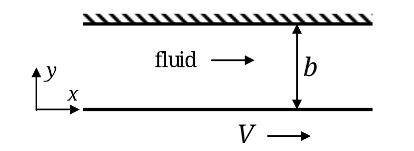
\includegraphics[width=0.5\columnwidth]{figs/qn 52 .jpg}
    \caption{}
    \label{fig:qn52.jpg}
\end{figure}
\item The steady, laminar velocity profile in the $x$-direction is
\hfill{\brak{\text{CH 2012}}}
\begin{enumerate}
\begin{multicols}{2}
    \item $V \left[\frac{y}{b}\right]$
    \item $V \left[\left(\frac{y}{b}\right)^2 - 1\right]$
    \item $V \left[1-\left(\frac{y}{b}\right)^2\right]$
    \item $V \left[1-\frac{y}{b}\right]$
    \end{multicols}
\end{enumerate}

\item The force per unit area (in the $x$-direction) that must be exerted on the bottom plate to maintain the flow is
\begin{enumerate}
\hfill{\brak{\text{CH 2012}}}
\begin{multicols}{4}
    \item $\mu V/b$
    \item $-\mu V/b$
    \item $2\mu V/b$
    \item $-2\mu V/b$
    \end{multicols}
\end{enumerate}

\section*{Statement for Linked Answer Questions 54 and 55:}

The first order liquid phase reaction $A \rightarrow P$ is conducted isothermally in a plug flow reactor of 5 liter volume. The inlet volumetric flow rate is 1 liter/min and the inlet concentration of A is 2 mole/liter.

\item If the exit concentration of A is 0.5 mole /liter, then the rate constant, in $\text{min}^{-1}$, is
\hfill{\brak{\text{CH 2012}}}
\begin{enumerate}
\begin{multicols}{4}
    \item $0.06$
    \item $0.28$
    \item $0.42$
    \item $0.64$
    \end{multicols}
\end{enumerate}

\item The plug flow reactor is replaced by 3 mixed flow reactors in series, each of 2.0 liters volume. The exact conversion of A (in $\%$) is
\hfill{\brak{\text{CH 2012}}}
\begin{enumerate}
\begin{multicols}{4}
    \item $35.9$
    \item $52.5$
    \item $73.7$
    \item $94.8$
    \end{multicols}
\end{enumerate}

\section*{General Aptitude (GA) Questions}
Q. 56 -- Q. 60 carry one mark each.

\item Which one of the following options is the closest in meaning to the word given below?
     \textbf{Mitigate}
     \hfill{\brak{\text{CH 2012}}}
    \begin{enumerate}
    \begin{multicols}{4}
        \item Diminish
        \item Divulge
        \item Dedicate
        \item Denote
    \end{multicols}
    \end{enumerate}

\item Choose the most appropriate alternative from the options given below to complete the following sentence:

Despite several \underline{\hspace{1cm}} the mission succeeded in its attempt to resolve the conflict.
\hfill{\brak{\text{CH 2012}}}
    \begin{enumerate}
    \begin{multicols}{4}
        \item attempts
        \item setbacks
        \item meetings
        \item delegations
        \end{multicols}
    \end{enumerate}

\item The cost function for a product in a firm is given by $5q^2$, where $q$ is the amount of production. The firm can sell the product at a market price of $50$ per unit. The number of units to be produced by the firm such that the profit is maximized is
\hfill{\brak{\text{CH 2012}}}
    \begin{enumerate}
    \begin{multicols}{4}
        \item $5$
        \item $10$
        \item $15$
        \item $25$
        \end{multicols}
    \end{enumerate}

\item Choose the most appropriate alternative from the options given below to complete the following sentence:
    
    Suresh's dog is the one \underline{\hspace{1cm}} was hurt in the stampede.
    \hfill{\brak{\text{CH 2012}}}
    \begin{enumerate}
    \begin{multicols}{4}
        \item that
        \item which
        \item who
        \item whom
        \end{multicols}
    \end{enumerate}

\item Choose the grammatically INCORRECT sentence:
\hfill{\brak{\text{CH 2012}}}
    \begin{enumerate}[label=(\Alph*)]
        \item They gave us the money back less the service charges of Three Hundred rupees.
        \item This country's expenditure is not less than that of Bangladesh.
        \item The committee initially asked for a funding of Fifty Lakh rupees, but later settled for a lesser sum.
        \item This country's expenditure on educational reforms is very less.
    \end{enumerate}

\section*{Q. 61 -- Q. 65 carry two marks each.}

\item An automobile plant contracted to buy shock absorbers from two suppliers X and Y. X supplies $60\%$ and Y supplies $40\%$ of the shock absorbers. All shock absorbers are subjected to a quality test. The ones that pass the quality test are considered reliable. Of X's shock absorbers, $96\%$ are reliable. Of Y's shock absorbers, $72\%$ are reliable.
    
    The probability that a randomly chosen shock absorber, which is found to be reliable, is made by Y is
    \hfill{\brak{\text{CH 2012}}}
    \begin{enumerate}
    \begin{multicols}{4}
        \item $0.288$
        \item $0.334$
        \item $0.667$
        \item $0.720$
        \end{multicols}
    \end{enumerate}

\item A political party orders an arch for the entrance to the ground in which the annual convention is being held. The profile of the arch follows the equation $y = 2X - 00.1X^2$ where $y$ is the height of the arch in meters. The maximum possible height of the arch is
\hfill{\brak{\text{CH 2012}}}
    \begin{enumerate}
    \begin{multicols}{4}
        \item $8$ meters
        \item $10$ meters
        \item $12$ meters
        \item $14$ meters
    \end{multicols}
\end{enumerate}

\item Wanted Temporary, Part-time persons for the post of Field Interviewer to conduct personal interviews to collect and collate economic data. Requirements: High School-pass, must be available for Day, Evening and Saturday work. Transportation paid, expenses reimbursed.
    
    Which one of the following is the best inference from the above advertisement?
    \hfill{\brak{\text{CH 2012}}}
    \begin{enumerate}
        \item Gender-discriminatory
        \item Xenophobic
        \item Not designed to make the post attractive
        \item Not gender-discriminatory
    \end{enumerate}

\item Given the sequence of terms, AD CG FK JP, the next term is
\hfill{\brak{\text{CH 2012}}}
\begin{enumerate}
\begin{multicols}{4}
    \item OV
    \item OW
    \item PV
    \item PW
    \end{multicols}
\end{enumerate}

\item Which of the following assertions are CORRECT?
\begin{itemize}
    \item[P:] Adding 7 to each entry in a list adds 7 to the mean of the list
    \item[Q:] Adding 7 to each entry in a list adds 7 to the standard deviation of the list
    \item[R:] Doubling each entry in a list doubles the mean of the list
    \item[S:] Doubling each entry in a list leaves the standard deviation of the list unchanged
    \hfill{\brak{\text{CH 2012}}}
\end{itemize}
\begin{enumerate}
\begin{multicols}{4}
    \item P, Q
    \item Q, R
    \item P, R
    \item R, S
\end{multicols}
\end{enumerate}
\centering
\textbf{END OF THE QUESTION PAPER}


\end{enumerate}
\end{document}